\section{Mispricing detection}
\label{sec:mispricing}

\subsection{Detectors}

A least-squares fit absorbs part of every mispriced quote into the surface. Each detector therefore
refits the day's \mixfour{} surface by iteratively reweighted least squares~\citep{holland1977} for a
Cauchy loss on residuals in half-spreads: a quote $u$ half-spreads from the surface has its
half-spread widened by $\sqrt{1+(u/c)^2}$, and the surface is refitted from the previous pass
(\cref{app:robust}). The traded detector, robust \mixfour, uses scale $c=1$ and two passes. A
mispriced segment of neighbouring strikes survives this refit, because each quote's weight reads
only its own residual and a smooth bump leaves each one small. The pooled robust detector therefore
weights each quote by the larger of its own residual and the mean residual over up to two strikes on
either side in its expiry ($c=0.25$, 16 passes), which down-weights a run of same-signed residuals as
a whole. It was chosen among 24 settings on Heston 2021 by the highest recall among settings at least
as precise as robust \mixfour. On the synthetic panels the cross-day model is a third detector: its
surface moves only through the latent, so it absorbs almost none of a mispricing.

Residuals are signed so that positive means the market is rich. A quote is flagged when the model
price lies outside the bid-ask by more than a margin $m$, in price half-spreads: rich quotes are sold
and cheap ones bought. Margins were chosen on the validation years: $m=0.5$ on synthetic data and
$m=4$ on SPX, where the conditional model is not used because its error is several times the
half-spread.

\subsection{Synthetic panels}

\Cref{tab:detection,fig:detection} score the detectors against the injected labels. Least-squares
fits absorb about half of a mispriced segment into the surface, and the robust refit barely changes
that (\robAbsorbFresh{} on the fresh panel); pooling cuts it to \segAbsorbFresh, and at the robust
detector's precision it adds 9 points of recall and 14 of segment recall. The conditional model
trained on nine years is the best detector on both test panels: precision \multiPrecFresh{} at recall
\multiRecFresh{} on the fresh panel, with \multiSegFresh{} of mispriced segments found, against
\robSegFresh{} for robust \mixfour{} and \segSegFresh{} for the pooled refit. Its precision is
0.995--0.998 in every quarter. The one-year model has the same recall but loses precision in two
quarters of each panel (0.35--0.52), where the variance leaves the range of its training year; in
2022Q4 its error against the true surface triples. Flagged residuals of the nine-year detector revert by
$-0.52$, $-0.95$ and $-0.99$ at 1, 3 and 5 days on Heston 2022, against an injected decay of $-0.50$,
$-0.875$ and $-0.97$.

\begin{table}[t]
  \centering\small
  \caption{Detection at margin 0.5 on the synthetic test panels, Heston 2022 / fresh panel. Labels are
  injected shifts above one half-spread; recall is split into isolated strikes and segments, and
  ``absorbed'' is the median share of a mispriced segment the detector's surface absorbs.
  Best values on the fresh panel in bold.}
  \label{tab:detection}
  \begin{tabular}{lrrrrr}
\toprule
& & \multicolumn{3}{c}{recall} & \\
\cmidrule(lr){3-5}
detector & precision & recall & isolated & segments & absorbed \\
\midrule
least-squares \texttt{mix4} & $0.902$ / $0.902$ & $0.39$ / $0.40$ & $0.53$ / $0.54$ & $0.21$ / $0.23$ & 56\% / 55\% \\
robust \texttt{mix4} & $0.954$ / $0.950$ & $0.44$ / $0.45$ & $0.58$ / $0.59$ & $0.27$ / $0.29$ & 53\% / 52\% \\
pooled robust \texttt{mix4} & $0.964$ / $0.964$ & $0.52$ / $0.54$ & $0.62$ / $0.64$ & $0.40$ / $0.43$ & 36\% / 34\% \\
conditional, one year & $0.635$ / $0.581$ & $0.63$ / $0.65$ & $\mathbf{0.63}$ / $\mathbf{0.65}$ & $0.63$ / $0.65$ & 4\% / 4\% \\
conditional, nine years & $\mathbf{0.997}$ / $\mathbf{0.996}$ & $\mathbf{0.63}$ / $\mathbf{0.65}$ & $0.63$ / $0.64$ & $\mathbf{0.62}$ / $\mathbf{0.66}$ & 4\% / 3\% \\
\bottomrule
\end{tabular}

\end{table}

\begin{figure}[t]
  \centering
  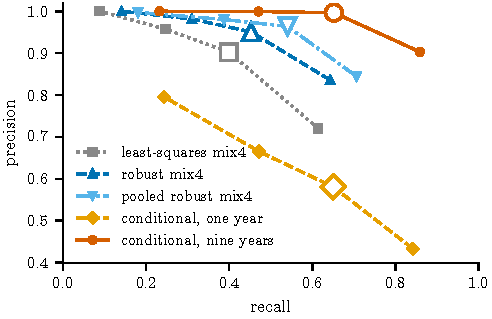
\includegraphics[width=0.54\linewidth]{detection.pdf}
  \caption{Precision against recall on the fresh synthetic panel as the margin falls from 2 to 0
  half-spreads; open circles mark the chosen margin 0.5.}
  \label{fig:detection}
\end{figure}

\subsection{Fitting failures and refits}
\label{sec:refits}

The first SPX runs used cached least-squares fits from the default start, and on some days that
start stops in a poor local minimum, in which the surface misses whole expiries. Such a day flags
many quotes that are not mispriced. The problem surfaced on 2016--2017, where 92\% of the cached-fit
flags fell on four days of October 2017. Every mispricing panel was therefore refitted: each day's
least-squares surface is the better, by its own objective, of the cached fit and a fit started from
the previous day's chosen surface, so days are fitted in date order, and the robust refits start
from it. This rule and every other setting were frozen on the validation years, together with a
written prediction of the outcome, before the test panels were run once more.

\Cref{tab:refit,fig:refit} show how often the cached fits failed. On \refitTwoX{} of the
\refitDays{} days of SPX 2023 the cached objective was more than twice what the surface can reach
(median ratio \refitMedian), and on the worst day of 2017 it was a hundred times higher. Validation
2022 and 2016 had milder failures, and the synthetic panels, drawn from one smooth model, had none.
On the validation years the refits changed little: the backtest selection rule again picked the
same margin and holding period, and the synthetic detection table is all but unchanged, so every
other setting was kept. The surface comparisons of \cref{sec:surfaces} fit \mixfour{} on their own
sampled days and were not rerun; minima there would overstate the mixture's fit error.

\begin{table}[t]
  \centering\small
  \caption{Least-squares objective of the chosen fit relative to the cached fit, per panel: days on
  which the previous-day start won, the median ratio, days with an objective more than 10\% and more
  than twice lower, and the worst day's objectives (mean squared IV residual in half-spreads).}
  \label{tab:refit}
  \begin{tabular}{lrrrrl}
\toprule
& & & \multicolumn{2}{c}{days lower by} & \\
\cmidrule(lr){4-5}
panel & start won & median & $>10\%$ & $>2\times$ & worst day \\
\midrule
SPX 2022 (validation) & 154 / 253 & $0.97$ & 54 & 0 & 0.47 $\to$ 0.25 (Sep 9) \\
SPX 2023 (test) & 205 / 247 & $0.69$ & 172 & 69 & 0.53 $\to$ 0.12 (Jul 7) \\
SPX 2016 & 105 / 251 & $1.00$ & 20 & 0 & 0.15 $\to$ 0.12 (Oct 27) \\
SPX 2017 & 144 / 250 & $0.96$ & 83 & 12 & 5.51 $\to$ 0.05 (Oct 24) \\
Heston 2021 & 41 / 261 & $1.00$ & 0 & 0 & -- \\
Heston 2022 & 48 / 234 & $1.00$ & 0 & 0 & -- \\
Heston, fresh 2023 & 42 / 260 & $1.00$ & 0 & 0 & -- \\
\bottomrule
\end{tabular}

\end{table}

\begin{figure}[t]
  \centering
  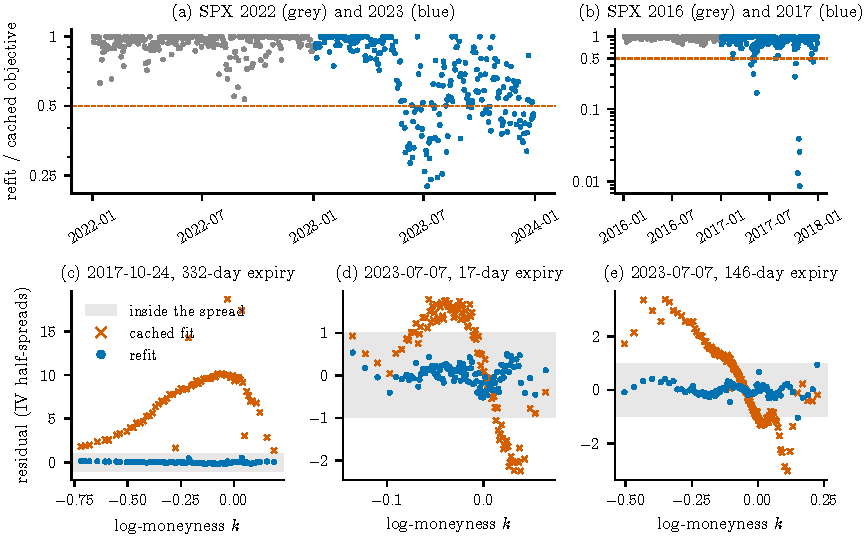
\includegraphics[width=\linewidth]{refit.pdf}
  \caption{(a, b) Refit-to-cached objective ratio per day (log scale); below the dashed line the
  cached fit was more than twice the reachable objective. (c--e) Residuals in IV half-spreads of the
  cached fit and the refit on (c) the SPX day with the largest reduction, October 24, 2017, at its
  expiry with the largest cached-fit error, and (d, e) the worst day of 2023 at its two such
  expiries; the shaded band is inside the spread.}
  \label{fig:refit}
\end{figure}

\subsection{Do flagged residuals revert?}

For each origin day and horizon $h$, the residual change of every contract quoted on both days is
regressed on its residual, separately for flagged and unflagged quotes; the daily slopes are averaged
and tested with Newey--West errors~\citep{fama1973,newey1987} (\cref{app:reversion}). A slope of
$-1$ is full reversion within $h$ days. Quote noise makes residuals revert even where nothing is
mispriced, so unflagged quotes are the control.

On the cached fits of SPX 2023, flagged residuals reverted faster than unflagged ones at every horizon
(\cref{tab:reversion}; $\revCachedDiffOne$ at one day, $p=\revCachedPOne$, on \revCachedDays{} days with at
least five flags). On the refits the robust detector flags 0.30\% of quotes (0.44\% before), with at
least five flags on \revDays{} days, and the one-day difference vanishes ($\revDiffOne$,
$p=\revPOne$). At 3 and 5 days a difference remains. The pooled detector's flags still revert faster
than unflagged ones at every horizon ($p<0.001$, \revSegDays{} days).

Reversion of a residual can come from either side: the market quote can move towards the surface,
or the surface, refitted each day, can move towards the quote. Only the first is a mispricing that
can be traded. With $x_t=(\sigma^{\text{mkt}}_t-\sigma^{\text{model}}_t)/s_t$ and $s_t$ the origin
day's IV half-spread, the slope of $x_{t+h}-x_t$ on $x_t$ splits exactly into the slope of the market
part minus that of the model part (\cref{app:reversion}). The lower block of \cref{tab:reversion}
shows the split. Neither detector's flagged prices move towards the model more than unflagged prices
do at one day ($p=\revMarketPOne$ for the robust detector). At 3 and 5 days the pooled detector's
flags revert mostly through the surface moving, and its flagged prices move significantly
\emph{less} towards the model than unflagged ones: distinguishable, but in the direction against a
tradable mispricing.

\begin{table}[t]
  \centering\small
  \caption{Reversion on SPX 2023 at margin 4. Upper block: flagged minus unflagged reversion slope of
  price residuals ($p$-values in parentheses; negative means flags revert faster). Lower block: slopes
  of IV residuals in origin-day half-spreads, split into the market's move and the model's; a
  positive model part is the surface moving towards the quote. The last rows test whether flagged
  prices move towards the model more than unflagged ones.}
  \label{tab:reversion}
  \begin{tabular}{lrrr}
\toprule
 & 1 day & 3 days & 5 days \\
\midrule
\multicolumn{4}{l}{\emph{reversion slope, price residuals, robust \texttt{mix4}}} \\
cached fits, flagged $-$ unflagged & $-0.23$ ($0.002$) & $-0.23$ ($<0.001$) & $-0.18$ ($0.003$) \\
refits, flagged $-$ unflagged & $-0.05$ ($0.72$) & $-0.24$ ($0.006$) & $-0.17$ ($0.05$) \\
\midrule
\multicolumn{4}{l}{\emph{IV residuals split into market and model moves (refits)}} \\
robust: flagged, market part & $-0.28$ ($0.17$) & $-0.53$ ($0.12$) & $-0.93$ ($0.02$) \\
robust: flagged, model part & $+0.01$ & $-0.04$ & $-0.57$ \\
robust: unflagged, market part & $-0.34$ & $-0.59$ & $-0.74$ \\
robust: market, flagged $-$ unflagged ($p$) & $0.89$ & $0.36$ & $0.72$ \\
pooled robust: flagged, market part & $-0.19$ ($0.13$) & $-0.08$ ($0.65$) & $-0.21$ ($0.36$) \\
pooled robust: flagged, model part & $+0.14$ & $+0.40$ & $+0.41$ \\
pooled robust: unflagged, market part & $-0.33$ & $-0.70$ & $-1.10$ \\
pooled robust: market, flagged $-$ unflagged ($p$) & $0.39$ & $<0.001$ & $<0.001$ \\
\bottomrule
\end{tabular}

\end{table}

\paragraph{The written prediction.} Before the test run we predicted that (i) the next-day reversion
of flags would mostly not be the market moving, and (ii) the flagged market move would not be
distinguishable from the unflagged one. Part (i) was not borne out at one day: most of the flagged
residuals' one-day change is the market's (robust $-0.28$ of $-0.29$; pooled $-0.19$ of $-0.33$),
though neither part is significant. At 3 and 5 days it holds for the pooled detector. Part (ii) holds
for robust \mixfour{} at every horizon and for the pooled detector at one day; at 3 and 5 days the
pooled detector's flagged prices are distinguishable, but they move less towards the model.

\subsection{Backtest}

Each flag of the traded detector is traded with \$1{,}000 of vega, crossing the spread on entry and
exit and paying \$1 per contract per side. It is delta-hedged daily with its expiry's forward and
closed once its residual is below half a spread, or after five days (\cref{app:backtest}). Next-day
execution, with the signal at one close and the trade at the next, is the main case; same-day
execution is an optimistic bound, since it assumes a fill at the closing quotes that produced the
signal. Each trade has 20 placebos: random unflagged contracts from the same day, type, direction and
maturity--moneyness bucket, held for the same days. The placebos earn what the strategy's exposure
earns, such as the volatility risk premium on sold options~\citep{bakshi2003,carr2009}, without its
signal.

\begin{table}[t]
  \centering\small
  \caption{Delta-hedged backtest of the traded detector at margin 4, holding at most five days, with
  20 matched placebos per trade. Sharpe ratios are annualized from daily net PnL; ``placebo'' is the
  placebos' mean net and ``excess'' the strategy's net minus it, with a Newey--West $p$-value. The validation row
  is the cell chosen by the selection rule, so it is biased upward. The synthetic rows trade the
  one-year conditional detector; trading the true labels checks the accounting.}
  \label{tab:backtest}
  \begin{tabular}{lrrrrrrr}
\toprule
execution & trades & gross & costs & net & Sharpe & placebo & excess ($p$) \\
\midrule
\multicolumn{8}{l}{\emph{SPX 2023 test, refits}} \\
next day & 1{,}482 & $+$\$476k & \$184k & $+$\$292k & $0.99$ & $+$\$233k & $+$\$59k ($0.31$) \\
same day (bound) & 1{,}586 & $+$\$545k & \$176k & $+$\$368k & $1.63$ & $+$\$48k & $+$\$320k ($0.02$) \\
\midrule
\multicolumn{8}{l}{\emph{SPX 2023 test, cached fits}} \\
next day & 2{,}595 & $+$\$162k & \$354k & $-$\$192k & $-0.66$ & $-$\$292k & $+$\$100k ($0.09$) \\
same day (bound) & 2{,}883 & $+$\$421k & \$351k & $+$\$70k & $0.35$ & $-$\$353k & $+$\$423k ($0.002$) \\
\midrule
\multicolumn{8}{l}{\emph{SPX 2022 validation, refits}} \\
next day & 3{,}420 & $+$\$948k & \$771k & $+$\$178k & $0.14$ & $-$\$454k & $+$\$632k ($0.02$) \\
\midrule
\multicolumn{8}{l}{\emph{SPX 2016--2017 replication, refits}} \\
next day & 3 & $+$\$2 & \$2.2k & $-$\$2.2k & $-1.03$ & $-$\$1.4k & $-$\$781 ($0.45$) \\
same day (bound) & 4 & $-$\$2.7k & \$1.9k & $-$\$4.5k & $-1.06$ & $-$\$3.8k & $-$\$741 ($0.51$) \\
\midrule
\multicolumn{8}{l}{\emph{Heston 2022 test, conditional (one year)}} \\
next day & 3{,}091 & $+$\$998k & \$1.58m & $-$\$584k & $-5.39$ & $-$\$1.52m & $+$\$940k ($<0.001$) \\
same day (bound) & 3{,}329 & $+$\$2.12m & \$1.74m & $+$\$383k & $3.09$ & $-$\$1.69m & $+$\$2.07m ($<0.001$) \\
true labels, same day & 2{,}786 & $+$\$1.75m & \$1.54m & $+$\$206k & $1.92$ & $-$\$1.55m & $+$\$1.75m ($<0.001$) \\
\bottomrule
\end{tabular}

\end{table}

\Cref{tab:backtest} gives the results. The accounting passes its check: trading the true synthetic
labels at the signal's close makes money net of costs. On the refitted SPX 2023 panel the next-day
strategy nets \btNet{} (\btTrades{} trades, Sharpe \btSharpe), but placebos net \btPlacebo{} over the
same holding days, and the excess, \btExcess, is not significant ($p=\btP$). \btSold{} of the trades are
sales in a year in which implied volatility fell, so the profit is likely the volatility risk
premium. The same-day bound beats its placebos ($p=\btSameP$), which does not contradict the slope
test. Placebos are contracts with small residuals, whereas a flag sits at least four half-spreads
outside the bid-ask: if it reverts by the same fraction as an unflagged quote, it still moves several
times as many dollars. The slope test asks whether it reverts by a larger fraction, and at one day it
does not. On the cached fits the next-day strategy lost \btCachedNet{}, with an edge over placebos
that was not significant either ($p=\btCachedP$).

On 2016--2017 the refits leave almost nothing to flag. Spreads are wider and the mixture sits inside
them, so margin 4 is a two to three times larger deviation in vol points than in 2023: the robust
detector flags 0.003\% of quotes, at most two days have five flags, and the strategy makes
\btRepTrades{} trades. Unflagged residuals there revert by $-0.79$, $-0.85$ and $-0.88$ at 1, 3 and
5 days, against $-0.33$, $-0.45$ and $-0.51$ in 2023, closer to the synthetic panels, which suggests
that residuals inside the spread are mostly quote noise rather than persistent misfit.
